% simple.tex - simple Master's thesis sample
% $Id: simple.tex 309 2011-01-28 14:46:48Z vlado $
\documentclass[12pt]{dalcsthesis}
% to prepare draft version use option draft:
%\documentclass[12pt,draft]{dalcsthesis}
\usepackage{verbatim}
\usepackage{amssymb}
\usepackage{adjustbox}
\usepackage{tabularx}
\usepackage{algorithm2e}
%\usepackage{caption}
%\captionsetup[table]{skip=10pt}
\usepackage{graphicx}
\begin{document}
\mcs  % options are \mcs, \macs, \mec, \mhi, \phd, and \bcshon
\title{Feature Based adaptive motion model}
\author{Rohan Bhargava}
\defenceday{1}
\defencemonth{October}
\defenceyear{2013}
\convocation{January}{2014}

% Use multiple \supervisor commands for co-supervisors.
% Use one \reader command for each reader.

\supervisor{Dr. Thomas Trappenberg}
\supervisor{Dr. Mae Sato}
\reader{D. Odaprof}
\reader{A. External}
\providecommand{\tabularnewline}{\\}
\newcommand{\lyxdot}{.}
\nolistoftables
\nolistoffigures

\frontmatter

\begin{abstract}
We present a method to learn and adapt the motion model. The motion model can be influenced by environmental properties and is a crucial part of the navigation system.Examples are the drift that is accounted in the motion model can be different for carpets and tiles. The AUV can have a change in their motion model when they are moving from fresh water to sea water. Our algorithm is based on the Expectation Maximization Framework which help us to learn the right parameters for the model.
The Expectation Step is completed by particle filtering and smoothing. The Maximization step involves finding the parameters for the model.We use side sonar images to extract landmarks which can gives us position estimates to help us evolve our motion model.This leads to a better position estimate of the robot. 
We found that the our learning motion model adapted well to the change in parameters and had low localization error compared to static motion model. 
This algorithm eliminates the need for laborious and hand-tuning calibration process. The main significance of learning the motion model is to have better navigation algorithms and also its a step towards robots being able to adapt to environment without human intervention.
We validate our approach by recovering a good motion model when the density,temperature of the water is changed in our simulations. 
\end{abstract}

\begin{acknowledgements}
Thanks to all the little people who make me look tall.
\end{acknowledgements}

\mainmatter

\chapter{Introduction}
 





\section{Motivation}


The core of human environment interaction is the ability of a person to know its position in surrounding environment. The process of estimating robot's position and orientation in the world is termed as Localization \cite{thrun2005probabilistic}. It is the answer to the question “Where am I?”. The current location of a robot can be determined by Global Positioning Systems, landmarks, maps etc. A common approach is to provide a prior map of the environment and a robot with help of sensors perceives the world and localizes itself in it. Another way to estimate the position of a robot is by knowing how a robot moves in the world . For example by knowing at what velocity a robot is moving we can predict its future location. There are various algorithms such as Particle Filter \cite{gordon1993novel},Kalman Fitler \cite{kalman1960new} etc. to estimate the state of a robot. The way the robot moves and senses the world are captured in motion and sensor models. These models are basic building blocks to various 
algorithms such 
as path planning \cite{Lav06}, Simultaneous Localization and Mapping (SLAM) \cite{thrun2005probabilistic} \cite{grisettiyz2005improving}  etc. which require an accurate estimate of robot's position.

In order to account for the uncertainty in the environment Sebastian Thrun \cite{thrun2005probabilistic} represented the models probabilistically. Eliazar and Parr \cite{Eliazar2004} pointed out that the essential input are the parameters to these models. The process of determining the parameters to a kinematic model is termed as calibration. Generally the robot is calibrated at the start of the experiment and the parameter values are not changed throughout the experiment. In practice wherever there is a significant change in the environment, robots are manually re calibrated during the experiment. In most of the cases it is not possible to recalibrate while the robot is in operation. As our environments are dynamic our models need to adapt to them. Eliazar and Parr \cite{Eliazar2004} proposed an algorithm to learn parameters of a motion model for land robots. Teddy Yapp \cite{Yap2008} took the work further and learned parameters for motion and sensor models for land robots. Both of their algorithms used 
Expectation Maximization framework to learn right parameters for models.

For my thesis I specifically deal with water environments such as oceans, rivers etc. which are highly dynamic and will lead to changes in motion model for Autonomous Underwater Vehicle. A specific application to demonstrate the importance of accurate motion model is Navigation. In AUV navigation relies on Inertial Navigation System(INS) which gives an estimate of velocity, position and orientation. All INS systems suffer from drift i.e. small errors in measurement of acceleration and angular velocity are integrated into progressively into larger error. Hegrenaes et al \cite{Hegrenes2008} pointed out that systems such as Doppler Velocity Log(DVL), surface GPS etc are used to compensate for the drift but they are situations where these systems fail or readings are discarded due to poor quality. To solve this particular problem they used velocity estimate from a static motion model to aid INS systems. In my thesis I propose an online system for an AUV to adapt its motion model to the dynamic environment which 
can be used for applications such as navigation as well as automate the calibration process. 

In Chapter~\ref{learning the motion model} I demonstrate how the parameters of a motion model can be estimated during its normal operation. The algorithm uses machine learning methods to learn the parameters as well as eliminate the necessity of identifying the parameters through a manual laborious calibration process. Yapp \cite{Yap2008} in his algorithm used Expectation Maximization \cite{dempster1977maximum} framework to estimate the right parameters for the model and I use the same framework for my algorithm. It is an unsupervised machine learning technique primarily used to estimate parameters. It alternates between the Expectation Step which creates an expectation of the log-likelihood using the current estimate of the parameters and the Maximization Step which computes parameters maximizing the expected log-likelihood found in the E step. 

In the algorithm proposed by Yapp \cite{Yap2008} to calculate the likely trajectory of a robot particle filtering \cite{ristic2004beyond} \cite{chen2003bayesian} and smoothing \cite{doucet2000monte} \cite{doucet2009tutorial} were performed using the sensor data collected during robot's normal operation. The particle filters were chosen because they can model non-linear transformations as well as they have no restrictions in model. Particle smoothing was performed because Russel and Norving \cite{russell2003artificial} pointed out the state of the system is better estimated by smoothing as it incorporates more information than just filtering. The maximum likelihood estimate of the parameters given the robot's trajectory and the motion data is calculated. The algorithm by Yapp \cite{Yap2008} was for land robots as well as assumed a prior map of the environment.  

The algorithm proposed in this thesis is for an AUV and can learn the motion model in unknown environments. In the algorithm instead of using a static map we used landmarks. In AUV the landmarks are extracted from side sonar images and are collected as sensor data. The algorithm assumes that the robot is equipped with a side sonar sensor and has access to its noisy motion data. Sound Navigation and Ranging (SONAR) is a technique based on sound propagation used for detecting objects underwater. The SONAR sensor is the only imaging tool which can work at high depth. Side scan sonar is a specific type of sonar used to image the topography of the sea floor.

To summarize I am proposing an algorithm to learn the right parameters of a motion model for an AUV. The parameters are learned on the fly without having a prior map or revisiting places. Results of the simulated experiment are presented in chapter ~\ref{results} to show the effectiveness of the algorithm. 
 

\section{Contributions}
The main contributions of the algorithm are-:

1) \textbf{Adaptive Motion Model}-: The motion model for AUVs adapt to changing environment. This automated process of calibration of the robots lead to no hand tuning of the models and gives us an online process which can be preformed during the robot's mission.  

2) \textbf{Motion Estimation from Side Sonar Images}-: We present an approach to estimate the movement from side sonar images which can be coupled with existing motion model and can improve localization. It can be easily be performed on-board as limited amount of interest points are used which lead to lesser computation and memory usage. 

\chapter{Background}
In the chapter we start by discussing how motion models are probabilistically represented as well as give an insight about motion models for AUV. This helps us in understanding on how motion model captures the probabilistic movements of robots. We then discuss a probabilistic state estimation algorithm i.e. Particle Filter \cite{ristic2004beyond} \cite{chen2003bayesian} which is at the heart of my algorithm as well as many other robotics systems. Lastly we discuss in detail about Particle smoothing \cite{doucet2000monte} \cite{doucet2009tutorial} which gives an estimate of ground truth by calculating the distribution of past states with taking into account all the evidence up to present. 

\section{Motion Model}
A motion model is responsible for capturing the relationship between the control input and the change in robot's configuration. Thrun \cite{thrun2005probabilistic} models the motion of a robot probabilistically because the same
control inputs will never reproduce the same motion. A good motion model will capture the errors such as drift that are encountered during the motion of the robot. The motion model is an integral part of algorithms such as localization,mapping etc. 

Let $X=(x,y,\theta)$ be the initial pose of the robot in x-y space. Mathematically the motion model can be described as $P(X^{'}|X,u)$, where $X^{'}$ is the pose after executing the motion command $u$. Based on the control input Thrun \cite{thrun2005probabilistic} divided the motion model in two classes 1) Odometry based motion model 2) Velocity based motion model.

The first class of motion models are used for robots equipped with wheel encoders. Odometry is generally obtained by integrating wheel encoders information and is more accurate than velocity.  
Velocity based models calculate the new position based on velocities and time elapsed. These models are implemented for Autonomous Underwater Vehicle(AUV) and Unmanned Aerial Vehicles(UAV). Both odometry as well as velocity suffer from drift and slippage therefore the same control commands will not generally produce the same motion and the motion model $P(X^{'}|X,u)$ is represented as probability distribution.

The velocity motion model proposed by Thrun \cite{thrun2005probabilistic} assumes that robot can be controlled through two velocities a rotational and translational velocity. The translational velocity at time $t$ is denoted by $v_{t}$ and rotational velocity by $w_{t}$. Hence the control input $u_{t}$ can be represented by  
\begin{center}
$u_{t}=\bigl(\begin{array}{c}
                v_{t} \\
                w_{t}
               \end{array}\bigr)$
  
\end{center}

The assumption is that positive rotational velocities $w_{t}$ induce a counterclockwise rotation whereas postive translational velocites $v_{t}$ correspond to forward motion. The set of equations to compute the next state of a robot for a velocity motion model are 
\begin{center}
$x_{t}=x_{t-1}+V_{t-1}/W_{t-1} \sin(\theta_{t-1})+ V_{t-1}/W_{t-1} \cos(\theta_{t-1} + W_{t-1} \delta t)$

$y_{t}=y_{t-1}+V_{t-1}/W_{t-1} \cos(\theta_{t-1})- V_{t-1}/W_{t-1} \sin(\theta_{t-1} + W_{t-1} \delta t)$

$\theta_{t}=\theta_{t-1}+ W_{t-1} \delta t$
 
\end{center}
%Read about the mathematical derivation for the equation

In an AUV a velocity motion model is implemented and to represent AUV's motion, 6 independent coordinates are necessary to determine the position and orientation of the rigid body. The notations used for marine vehicles are described in Table \ref{marine notation}. 
%\begin{center}

\begin{table}
\label{marine notation}
\caption{Notation used for marine vehicles}

\begin{tabular}{|c|>{\centering}p{3cm}|>{\centering}p{3cm}|>{\centering}p{3cm}|>{\centering}p{3cm}|}
\hline 
DOF &  & forces and moments & linear and angular vel. & positions and Euler angles\tabularnewline
\hline 
\hline 
1 & motions in the x-direction (surge) & X & u & x\tabularnewline
\hline 
2 & motions in the y-direction (sway) & Y & v & y\tabularnewline
\hline 
3 & motions in the z-direction (heave) & Z & w & z\tabularnewline
\hline 
4 & rotation about the x-axis (roll) & K & p & $\phi$\tabularnewline
\hline 
5 & rotation about the y-axis (pitch) & M & q & $\theta$\tabularnewline
\hline 
6 & rotation about the z-axis (heave) & N & r & $\psi$\tabularnewline
\hline 
\end{tabular}

\end{table}

%\end{center}



The pose of AUV can be represented as $s=(x,y,z,\theta,\phi,\psi)$. The first three coordinates correspond to the position along the x,y,z axes while the last three coordinates describe the orientation.


To estimate the position of an AUV we need to calculate the velocity at which the AUV is currently moving. The velocity can be computed in two ways-: 1) Static Motion model 2) Dynamic Motion model

Hegrenaes \cite{Hallingstad2007} points that a way to implement a simple static motion model as table look-up based on experimental data. 
\begin{center} $u_{r}=f(n_{s})$ \end{center} 
$u_{r}$, $n_{s}$ are the water relative linear velocity in x direction and control system set point respectively. In a similar manner an expression can be established for $v_{r}$.

Another way to implement the motion model is through dynamics. The 6 Degrees of Freedom (DOF) rigid body equations of motion described by Fossen \cite{Thor} are \\

$X=m[u^{.}-vr+wq-x_{G}(q^{2}+r^{2})+y_{G}(pq-r^{.})+z_{G}(pr+q^{.})]$

$Y=m[v^{.}-wp+ur-y_{G}(r^{2}+p^{2})+z_{G}(qr-p^{.})+x_{G}(qp+r^{.})]$

$Z=m[w^{.}-uq+vp-z_{G}(p^{2}+q^{2})+x_{G}(rp-q^{.})+y_{G}(rq+p^{.})]$

$K=I_{x}p^{.}+(I_{z}-I_{y})qr-(r^{.}+pq)I_{xz}+(r^{2}-q^{2})I_{yz}+(pr-q^{.})I_{xy}+m[y_{G}(w^{.}-uq+vp)-Z_{g}(v^{.}-wp+ur)]$

$M=I_{y}q^{.}+(I_{x}-I_{z})rp-(p^{.}+qr)I_{xy}+(p^{2}-r^{2})I_{zx}+(qp-r^{.})I_{yz}+m[y_{G}(u^{.}-vr+wq)-z_{g}(w^{.}-uq+vp)]$

$N=I_{z}r^{.}+(I_{y}-I_{x})pq-(q^{.}+rp)I_{yz}+(q^{2}-p^{2})I_{xy}+(rq-p^{.})I_{zx}+m[x_{G}(v^{.}-wp+ur)-y_{g}(u^{.}-vr+wq)]$

% need to find the best way to write these equations
\begin{figure}[hbtp]
\caption{Body-fixed reference frames}


\includegraphics[scale=0.8]{/home/rohan/Documents/thesis_work/uav_diagram.png}

\end{figure}

The equations described above can be expressed in a more compact form: 
% what is RB
\begin{equation}
\label{eq:motion model AUV}
M_{RB}\mathcal{{V}}^{.}+C_{RB}(\mathcal{V})\mathcal{V}=\tau_{RB}%
\end{equation}

Here $\mathcal{V}=[u,v,w,p,q,r]^{T}$ is the body fixed linear and angular velocity and $\tau_{RB}=[X,Y,Z,K,M,N]$ is generalized vector of external forces and moments. $M_{RB}$ is the rigid body inertia matrix and $C_{RB}$ is Coriolis and centripetal matrix. 

The right hand side of the vector \ref{eq:motion model AUV} represents the external forces and moments acting on the vehicle. Fossen \cite{Thor} classifies the forces into-:
\begin{itemize}
\item Radiation-induced forces

\begin{itemize}
\item added inertia
\item hydrodynamic damping
\item restoring forces
\end{itemize}
\item Environmental Forces

\begin{itemize}
\item Ocean currents
\item Waves

\end{itemize}
\item Propulsion Forces

\begin{itemize}
\item Thruster/Propeller Forces
\item Control Surfaces/Rudder Forces
\end{itemize}
\end{itemize}

$\tau_{RB}$ can be represented as 
\begin{equation}
\label{eq:total forces}
 \tau_{RB} = \tau_{H} + \tau_{E} + \tau 
\end{equation}

Here $\tau_{H}$ is the radiation induced forces and moments, $\tau_{E}$ is used to describe the environmental forces and moments and $\tau$ is the propulsion forces and moments. Equations \ref{eq:motion model AUV} and equation \ref{eq:total forces} can be combined to yield the following representation of 6 DOF dynamic equations of motion:
 
\framebox{\begin{minipage}[t]{1\columnwidth}%
\begin{equation}
\label{eq:vehicle hydrodynamics}
M\mathcal{{V}}^{.}+C(\mathcal{V})\mathcal{V}+D(\mathcal{V})\mathcal{V}+g(\eta)=\tau_{E}+\tau%
\end{equation}

\end{minipage}} \\

where 

$M \triangleq M_{RB} + M_{A}$ ; $C(\mathcal{V}) \triangleq C_{RB}(\mathcal{V} + C_{A}(\mathcal{V})$

$M_A$ is the added inertia  matrix $C_{A}(\mathcal{V})$ is the matrix of hydrodynamic Coriolis and centripetal terms. $g(\eta)$ is the restoring force.

Lammas \cite{Lammas2004} pointed out that navigation equation of an underwater vehicle is-:

\begin{equation}
\label{navigation equation for AUV}
\mathcal{V}^{.} = M^{-1}(\tau-C(\mathcal{V})\mathcal{V}-D(\mathcal{V})\mathcal{V}-g(\eta))
\end{equation}


$\mathcal{V}^{.}$ can be integrated with time to get velocity.

In the static model the velocity is calculated from a lookup table. In the other model we are computing forces and moments on the fly but the parameters to these forces are considered to be static. The parameters such as density, temperature etc of water can change with time and lead to an inaccurate estimate of velcoity in both the models. Hence the velocity needs to be adapted and Chapter \ref{adapting the motion model} explains how it is done in my algorithm.    


\begin{comment}
The 6-DOF rigid body equations of motions are 

$X=m[u^{.}-vr+wq-x_{G}(q^{2}+r^{2})+y_{G}(pq-r^{.})+z_{G}(pr+q^{.})]$


$Y=m[v^{.}-wp+ur-y_{G}(r^{2}+p^{2})+z_{G}(qr-p^{.})+x_{G}(qp+r^{.})]$

$Z=m[w^{.}-uq+vp-z_{G}(p^{2}+q^{2})+x_{G}(rp-q^{.})+y_{G}(rq+p^{.})]$

$K=I_{x}p^{.}+(I_{z}-I_{y})qr-(r^{.}+pq)I_{xz}+(r^{2}-q^{2})I_{yz}+(pr-q^{.})I_{xy}+m[y_{G}(w^{.}-uq+vp)-Z_{g}(v^{.}-wp+ur)]$

$M=I_{y}q^{.}+(I_{x}-I_{z})rp-(p^{.}+qr)I_{xy}+(p^{2}-r^{2})I_{zx}+(qp-r^{.})I_{yz}+m[y_{G}(u^{.}-vr+wq)-z_{g}(w^{.}-uq+vp)]$

$N=I_{z}r^{.}+(I_{y}-I_{x})pq-(q^{.}+rp)I_{yz}+(q^{2}-p^{2})I_{xy}+(rq-p^{.})I_{zx}+m[x_{G}(v^{.}-wp+ur)-y_{g}(u^{.}-vr+wq)]$

The first three equations represent the translational motion and the
last three represent the rotational motion.$X,Y,Z,K,M,N$ are the
external forces and moments of external forces. $u,v,w$ and $p,q,r$
represent the linear angular velocity of $X,Y,Z$ respectively. $x_{G},y_{G},z_{G}$
represents the center of gravity.

The above equations can be represented in a more compact and vectorial
form.




The forces acting on AUV can be broken down into three classes-:

The external forces and moments vector $\tau_{RB}$is the sum of the
forces listed above 

$\tau_{RB}=\tau_{H}+\tau_{E}+\tau$

Here $\tau_{H}$ is the radiation induced forces and moments, $\tau_{E}$
and $\tau$ are the environmental and propulsion forces and moments respectively. 
A standard numerical ODE integration routine can be used to solve the equation to recover the state.

The input to a motion model is a control command and in our case it is the velocity of the AUV. The velocity is calculated from the propellers. In our algorithm we assume a static model to get a velocity estimate. This can be implemented as a table look-up based on experimental data.
The same control input won't produce the same output every time as it is dependant upon the environment. Therefore we assume a Gaussian distribution over the velocity and try to learn the right parameters over time. 
For my master's thesis we reduce the degrees of freedom and represent the pose of the AUV is two dimensional with orientation. 

In the algorithm the robot can be represented by $X_{t}=(x_{t},y_{t},\theta_{t})$
where $x_{t},y,\theta_{t}$ are the robot's coordinates in x and y
plane and orientation at time $t$. We base our motion model equations on Teddy N. Yap motion model which specifically dealt with odometry to update the pose of the robot. In the set of equations for our model we replace the odometry with velocity. 

$x_{t}=x_{t-1}+V_{t-1}/W_{t-1} \sin(\theta_{t-1})+ V_{t-1}/W_{t-1} \cos(\theta_{t-1} + W_{t-1} \delta t)$

$y_{t}=y_{t-1}+V_{t-1}/W_{t-1} \cos(\theta_{t-1})- V_{t-1}/W_{t-1} \sin(\theta_{t-1} + W_{t-1} \delta t)$

$\theta_{t}=\theta_{t-1}+ W_{t-1} \delta t$


The terms $V_{t}$ and $W_{t}$are the translational and rotational
velocities respectively. They are represented by a Gaussian distribution
to account for the change in forces. They can mathematically represented
as 

$V_{t}\sim\mathcal{{N}}(v_{t},v_{t}^{2}\sigma_{V_{v}}^{2}+w_{t}^{2}\sigma_{V_{w}}^{2}+\sigma_{V_{1}}^{2})$

$W_{t}\sim\mathcal{{N}}(w_{t},v_{t}^{2}\sigma_{w_{v}}^{2}+w_{t}^{2}\sigma_{V_{w}}^{2}+\sigma_{W_{1}}^{2})$

In the above equations $v_{t}$ and $w_{t}$are reported translational
and rotational velocity. $\sigma_{A_{b}}$ describes the contribution
of velocity term b to the variance of the distribution over A. $\sigma_{V_{1}}$and
$\sigma_{W_{1}}$ take into account the independent errors that are
not proportional to translation and rotation of the robot. $\sigma_{V_{v}}^{2}\ensuremath{,}\sigma_{W_{v}}^{2}\ensuremath{,}\sigma_{V_{w}}^{2}\ensuremath{,}\sigma_{W_{w}}^{2}\ensuremath{,}\sigma_{V_{1}}^{2}\ensuremath{,}\sigma_{W_{1}}^{2}$
are the motion parameters that our algorithm intends to learn.
\end{comment}

\section{Particle Filter}
Particle Filter is a state estimation algorithm based on a sampling method for approximating a distribution. Thrun \cite{thrun2005probabilistic} defines particle fitler as an alternative non-parametric implementation of the Bayes filter. It also can be called as a Sequential Monte Carlo(SMC) algorithm. The first attempt to use SMC was seen in simulations of growing polymers by M.N Rosenbluth and A.W. Rosenbluth \cite{rosenbluth1955monte}. Gordon et al. \cite{gordon1993novel} provided the first true implementation of sequential monte carlo algorihtm. 
\begin{comment}
Advantages write  after all introdcution of particle filter

Particle Filters have no restrictions in model i.e. it can be applied to non-Gaussian models,they are super set of other filtering methods i.e. Kalman filter is Rao-Blackwellized particle filter with one particle.Additionally they can model non linear transformations of random variables therefore can be applied to any system and measurement models. All the advantages make them a good alternative to Extended Kalman Filter(EKF) and Unscented Kalman Filter(UKF).
\end{comment}

\begin{figure}[hbtp]
\caption{Markov Chain}
\centering
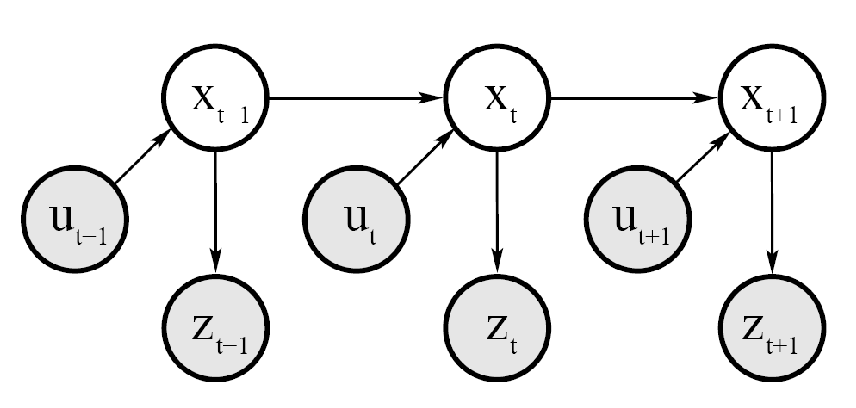
\includegraphics[scale=0.5]{../../thesis_work/markov_chain.png}
\end{figure}
Thrun \cite{thrun2005probabilistic} stated that the key idea behind particle filter is to represent the posterior bel$(x_{t})$ by a set of random state samples drawn from this posterior. Instead of representing the distribution by a parametric form particle filter represents a distribution by a set of samples drawn from this distribution. The representation is a approximation but it is nonparametric and therefore there are advantages of using particle filters as an alternative to Extended Kalman Filter and Unscented Kalman Filter. Particle Filters can represent a broader space of distributions for example non-Gaussians and can model non linear transformations of random variables. 

\begin{figure}[hbtp]
\caption{The ``particle'' representation used by particle filters. The lower upper right graphs shows samples drawn from a Gaussian random variable, X. These samples are passed through the nonlinear function shown in the upper right graph. The resulting samples are distributed according to the random variable Y.}
\centering
\includegraphics[scale=0.5]{/home/rohan/Documents/thesis_work/particle_filter_non_gaussian_thrun.png}
\end{figure}

%this figure is copied from Thrun.. How do I reference it???%

The algorithm for particle filters \cite{thrun2005probabilistic} is described below-:

\begin{algorithm}[H]
\label{alg:ParticleFilter}
 \SetAlgoLined
  		 
 \KwIn{$ X _{t-1}$: particle set \\
 $u_{t}$: most recent control \\
 $z_{t}$: most recent measurement}


 \KwOut{ $X_{t}$:particle set }
\Begin{
\For { m=1 to M do} 
{sample $x_{t}^{m}~p(x_{t}|u_{t},x_{t-1}^m)$
$w_{t}^{m}=p(z_{t}|x_{t}^{m})$
$X_{t}^{-}=X_{t}^{-}+(x_{t}^{m},w_{t}^m)$}

\For{m=1 to M do}
{
draw $i$ with probability $\propto$ $w_{t}^{[i]}$
\\
add $x_{t}^{[i]}$ to $X_{t}$}
return $X_{t}$
}
\caption{Particle Filter Algorithm}
\end{algorithm}

In algorithm ~\ref{alg:ParticleFilter} each particle $x_{t}^{m}$ is instantiation of the state at time $t$.  The first step is to generate a hypothetical state $x_{t}^{m}$ for time $t$ based on previous state $x_{t-1}^{m}$ and control $u_{t}$. The particles are samples from the state transition distribution $p(x_{t}|u_{t},x_{t-1})$. The importance factor for each particle $x_{t}^{m}$ is calculated and denoted by $w_{t}^{m}$. Importance factor is defined as the probability of measurement $z_{t}$ under the particle $x_{t}^{m}$. Thus importance factor are used to incorporate the measurements into the particle set. In practice, the number of particles used are a large number(e.g.-:1000).

The key part of the algorithm is the re-sampling step in particle filter algorithm. The algorithm draws M particles with replacement from a temporary particle set $X_{t}^{-}$. The probability of drawing the particles is given by the importance factor. The re-sampling step is a probabilistic implementation of the Darwinian idea of survival of the fittest. It refocuses the particle set to regions in state space with high posterior probability. 

Particle Filters is an integral part of my algorithm to learn the right parameters of the motion model and the way it is used is explained in ~\ref{ch:adapting the motion model}.

\section{Particle smoothing}
The particle filter algorithm as described before is the first step in the Expectation process. The next algorithm that completes the Expectation Step is the particle smoothing. Doucet \cite{doucet2009tutorial} in his paper stated that filtering based on observations recieved up to the current time is used to estimate the distribution of the current state of an Hidden Markov Model (HMM) whereas smoothing is used to estimate distribution of state at a particular time given all the observations up to some later time. Russel and Norving \cite{russell2003artificial} showed that the state of the system is better estimated by smoothing as it incorporates more information than just filtering. We use particle smoothing algorithm proposed by Teddy N Yap and Christian R. Shelton \cite{Yap2008} which was based on the technique presented by Docuet et al. \cite{doucet2000monte} and Godsill et al. \cite{Godsill2004}.

Algorithm ~\ref{alg:Particle Smoothing} is used to generate samples from the entire joint smoothing density $p(x_{0:T}|u_{1:T},z_{1:T})$.

\begin{algorithm}[H]
 \SetAlgoLined
  	\label{alg:Particle Smoothing}
 \KwIn{$ X _{t}, t = 0, 1, ..., T$: particle approximations to the posterior pdfs $p (x _{t}|c _{1:t}, s _{1:t}) , t = 0, 1, ..,T$ 
\\
$c _{1:T} = (c _{1}, c _{2}, ..., c _{T} )$: set of controls from time 1 to time T}
 \KwOut{ $x ^{'} _{0:T} = (x ^{'}_{0},x ^{'}_{1}, ...,x^{'}_{T} )$: a sample from the entire joint smoothing density $p (x_{0:T} |c _{1:T} , s _{1:T} )$ }
\Begin{draw \textit{i} with probability $\propto$ $w ^{[i]} _{T}$
$x ^{'} _{T} \leftarrow x^{[i]}_{T}$
\\
\For {$t \leftarrow T-1$ down to 0 do}{\For{ $i \leftarrow 1 to N_{s}$ do}{$w ^{[i]}_{t|t+1} \leftarrow w ^{[i]} _{t}p(x ^{'} _{t+1}|u _{t+1})$}draw \textit{i} with probability $\propto w ^{[i]} _{t|t+1}$\\ $x{'} \leftarrow x^{[i]}_{t}$}}
	\caption{Sample the entire joint smoothing density $p(x_{0:T}|c_{1:T},s_{1:T})$}
	
\end{algorithm}

The technique assumes that particle filtering has already been carried on the dataset which results in a set of particles with their corresponding weights at the present time step. In the first step of smoothing we choose a particle with the probability proportional to the weight of the particles. The next step is to move a time step back and calculate the new smoothed weights which are the product of forward probability and the weight of the particle as shown in equation ~\ref{eq:smoothing}. The smoothed weights are calculated till time($t$) = 0.

\begin{equation}
\label{eq:smoothing}
p(x_{t}|x_{t+1:T},u_{1:T},z_{1:T})=p(x_{t+1}|x_{t},u_{t+1})p(x_{t}|u_{1:t},z_{1:t})
\end{equation}

To calculate the trajectory we draw particles according to the new smoothed weights. At every time step we pick a particle and add it our trajectory set till time=T. We can repeat this process any number of time to get several trajectories. These trajectories are treated as ground truth and help in estimating the parameters of motion model. 
 
 

\section{SURF}
It is a robust local feature detector, first proposed by Herbert Bay et al. in 2006. The sta

\chapter{Learning the motion model}
\label{learning the motion model}
\section{General Architecture}


\begin{figure}[hbtp]
\label{fig:general archi}
\caption{Block Diagram of the framework}
\centering
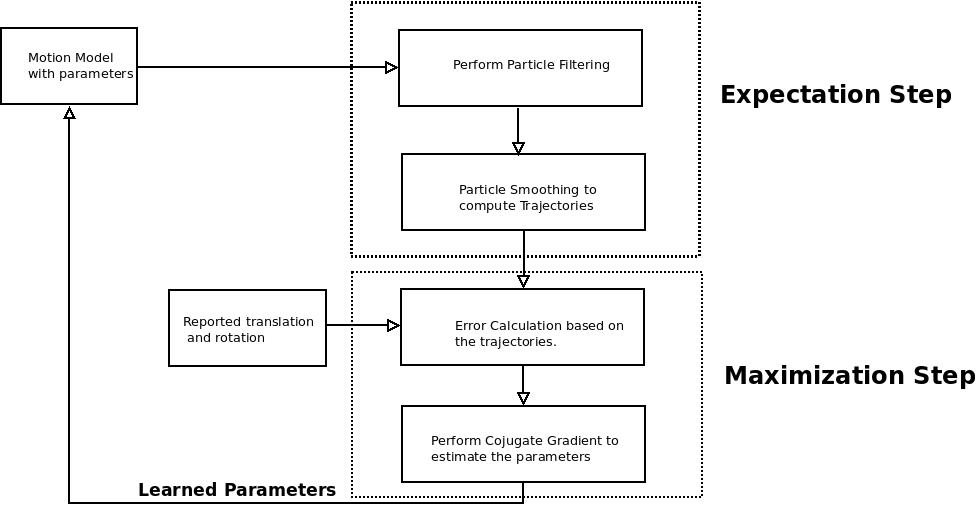
\includegraphics[scale=0.5]{Diagram1.jpeg}
\end{figure}



Figure ~\ref{fig:general archi} is a block diagram describing the whole system. The
first step is to initialize the motion model with a set of parameters.

Given the prior distribution $p(x_{t-1})$ of the robot's pose at time t-1,the motion model $p(x_{t}|x_{t-1},u_{t})$,the sensor model $p(z_{t}|x_{t})$,the control commands $u_{1:t}$ and the sensor measurements $z_{1:T}$ we perform particle filtering using Algorithm  ~\ref{alg:ParticleFilter} from time t=1 to time t=T. After we perform filtering we have a set of particles with importance factors describing the distribution over the pose of the robot.
To complete the Expectation Step particle smoothing is performed recursively backwards in time. A set of trajectories are generated by repeating Algorithm ~\ref{alg:Particle Smoothing}.


Based on the trajectories and the reported translational and rotational 
motion we calculate errors at each time step. We perform newton conjugate
gradient on the errors to give us the best estimate of the parameters.
This completes the Maximization Step.

The learned parameters are re-assigned to the motion model which helps in adapting the model. The  whole
process is repeated at each time step so that we can dynamically learn the right parameters. Various algorithm such as SLAM,Kalman Filter are dependent upon the accuracy of the motion model and adapting our motion models is the most basic step towards it. We found that the adaptive motion model performs better than the static and the results are shown in the later chapters.






\section{Dynamic Landmarks}
In the particle filtering algorithm the sensor model is responsible to assign weights to the particles.The sensor model describes the process by which sensor measurements are generated in the physical world.It is generally done by using some sort of references in the world aka landmarks. Austin and Elizar in their papers used static maps of known environments to generate references for their sensor model.
The probability of having static maps for underwater environments is pretty low and thus lead us to use side sonar images as references for the sensor model.
\begin{figure}[hbtp]
\caption{Side Sonar Image}
\centering
\includegraphics[scale=0.5]{/home/rohan/Documents/thesis_work/visual_sonar/sonar_59/18.jpg}
\end{figure}
As you can see in the image there are lot of horizontal lines which we treat as noise. For us to use the side sonar images we performed a pre-processing step in which we used a median filter on the image. This helped us in getting rid of major noises in terms of horizontal lines but also blurred the image. In order to generate some landmarks we ran feature extractions techniques like SURF. This algorithm helped us in detecting interest points in the image and are shown below in circles. Andrew Vardy{refer the paper) ran multiple image registration techniques such as phase matching (you need to mention more) on side sonar images and showed that SURF performs better than the rest .
\begin{figure}[hbtp]
\caption{SURF Keypoints}
\centering
\includegraphics[scale=0.4]{/home/rohan/Documents/thesis_work/visual_sonar/landmarks.png}
\end{figure}

These interest points can be treated as landmarks. We use a high Hessian
threshold so that we have a maximum of 4 landmarks. The distance of the robot and the particles to these landmarks are used to assign weights to the particles.
\\
The output of a side sonar is a ping of the surface and for an image to be created we need to combine pings over time. Andrew Vardy in his paper explains on how to combine pings to create an meaningful image. For our algorithm to run on the AUV we can use Andrew's algorithm as a black box and run our feature extraction on the output i.e. images of the seabed. 
This method allows us independence from a static map as well as helps in learning
the motion model on the fly in a new environment. 
\section{Adapting the motion model by parameter estimation}
\label{ch:adapting the motion model}

Velocity as distribution
As stated in earlier chapters as our environment changes the estimate for a control input becomes erroneous. The control input to a AUV's motion model is velocity and to adapt our motion motion we assume it as a Gaussian distribution. This chapter describes an algorithm to adapt the parameters for a distribution representing velocity. To adapt parameters of a distribution we use a Expectation Maximization \cite{dempster1977maximum} which is an unsupervised machine learning technique. 

Expectation Maximization is an iterative process of finding maximum likelihood of parameters of a model which depend upon hidden variables. We use the EM algorithm as described by Christopher M. Bishop in his book \cite{bishop2006pattern}. We have a joint distribution $p(X,Z|\theta)$ where X are the observed variables and Z are the latent variables governed by parameters $\theta$. The goal is to maximize the likelihood function $p(X|\theta)$ with respect to $\theta$. The steps taken in EM algorithm are described below -:

\\
1. Have an initial estimate of the parameters $\theta ^{old}$
\\
2. \textbf{E Step:} Evaluate $p(Z|X,\theta^{old})$
\\
3. \textbf{M Step:} Evaluate $\theta ^{new} = arg max _{\theta} L(\theta,\theta^{old})$
\\
\hspace*{20 mm} where 
$L(\theta,\theta^{old})=\Sigma _{Z} p(Z|X,\theta_{old}) \log p(X,Z|\theta)$
\\
4. Check for the convergence of either the log likelihood or the parameter values. If the convergence criterion is not satisfied then let
\\
\hspace*{20 mm} $\theta \leftarrow \theta^{new} $
\\
and return to step 2
\\
There are various convergence techniques that can be applied in step 4. In our algorithm we use Newton Conjugate Gradient to estimate the right parameters.	

%write about now you algorithm like in the Expecation Step in your algorihtm what you do%
% 3 dof , equations that are used to estimate the position%
% then you talk about the EM process with differences and all%


The first step of parameter estimation i.e. Expectation Step consists of particle filtering and smoothing as described in Chapters  and  respectively. The output of this step is a set of robot trajectories which are treated as ground truth. At each time step we calculate the error between the distance given by trajectory and the actual distance moved. 
\\
$\epsilon_{T_{t}}^{[j]}=(\theta_{t_{+1}}^{'[j]}-\theta_{t}^{'[j]}-r_{t}^{''})mod2\pi$ 
\\
$\epsilon_{D_{t}}^{[j]}=(x_{t+1}^{'[j]}-x_{t}^{'[j]})cos(\theta_{t}^{'[j]}+\frac{r_{t}^{''}+\epsilon_{T_{t}}^{[j]}}{2}+(y_{t+1}^{'[j]}-y_{t}^{'[j]})sin(\theta_{t}^{'[j]}+\frac{r_{t}^{''}+\epsilon_{T_{t}}^{[j]}}{2})-d_{t}^{''}$
\\
\\
$\epsilon_{T_{t}}^{[j]}$ and $\epsilon_{D_{t}}^{[j]}$ are rotational and translational errors for t=0,1...T-1 for $j^{th}$ sampled trajectory. $\epsilon_{W_{t}}^{[j]}$ and $\epsilon_{V_{t}}^{[j]}$ are the rotational and translation errors in velocity and is given by $\epsilon_{T_{t}}^{[j]}/\delta(t)$ and $\epsilon_{D_{t}}^{[j]}/\delta(t)$. $r_{t}^{''}$ and $d_{t}^{''}$ are the distance moved and are  given by $r_{t}^{''}=w_{t}*\delta(t)$ and $d_{t}^{''}=v_{t}*\delta(t)$. $w_{t}$ and $v_{t}$ are the reported velocity. 
Based on the motion model described 
\\
$\epsilon_{V_{t}}^{[j]}\sim\mathcal{{N}}(0,v_{t}^{2}\sigma_{V_{v}}^{2}+w_{t}^{2}\sigma_{V_{w}}^{2}+\sigma_{V_{1}}^{2})$
\\
$\epsilon_{W_{t}}^{[j]}\sim\mathcal{{N}}(0,v_{t}^{2}\sigma_{w_{v}}^{2}+w_{t}^{2}\sigma_{V_{w}}^{2}+\sigma_{W_{1}}^{2})$
\\
The log likelihood functions are
\\
$\mathcal{{L}}(\sigma_{V_{v}}^{2},\sigma_{V_{w}}^{2},\sigma_{V_{1}}^{2})=-\frac{1}{2}\sum_{j}\sum_{t=0}^{T-1}[\log2\pi+\log(v_{t}^{2}\sigma_{V_{v}}^{2}+w_{t}^{2}\sigma_{V_{w}}^{2}+\sigma_{V_{1}}^{2})+\frac{(\epsilon_{V_{t}}^{[j]})^{2}}{v_{t}^{2}\sigma_{V_{v}}^{2}+w_{t}^{2}\sigma_{V_{r}}^{2}+\sigma_{V_{1}}^{2}}$
\\
$\mathcal{{L}}(\sigma_{W_{v}}^{2},\sigma_{W_{w}}^{2},\sigma_{W_{1}}^{2})=-\frac{1}{2}\sum_{j}\sum_{t=0}^{T-1}[\log2\pi+\log(v_{t}^{2}\sigma_{W_{v}}^{2}+w_{t}^{2}\sigma_{W_{w}}^{2}+\sigma_{W_{1}}^{2})+\frac{(\epsilon_{W_{t}}^{[j]})^{2}}{v_{t}^{''2}\sigma_{W_{v}}^{2}+w_{t}^{''2}\sigma_{W_{w}}^{2}+\sigma_{W_{1}}^{2}}$
\\
\\
In the Maximization Step we minimize the likelihood function. In this
case we maximize the log likelihood function because of the minus
sign with respect to the motion parameters. We use newton conjugate
gradient ascent for finding the local maximum of the function. The
gradient of the function is the taken as the first search direction
while the next search direction are chosen in such a way that they
are orthogonal to all previous search directions.

The output of the step described above is a set of parameters that
maximize the function. We substitute these values in our motion model
at every time step and the process is repeated throughout the robot's
mission. 
\section{Visual Motion Estimates}
In AUV the motion estimation is generally done through dead-reckoning.
It is a process of calculating the current position based upon the
previous position and the speed of vessel. The velocity of the AUV
can be estimated by the acceleration measurement supplied by an Inertial
Measurement Unit. Another way is to use a Doppler Velocity Log(DVL) that
measures velocity in water by measuring the Doppler effect on scattered
sound waves. Dead reckoning may have significant errors as the velocity
and direction must be accurately known at every time step. 

In this algorithm we propose to get motion estimates using side sonar
images. As stated before we run SURF on the images and generate some
key points. These key points are matched in the next image using a
KNN based matcher. The matched key points gives us an estimate on
the movement of the vehicle. In the figure we show two consecutive
images and in the first image we have the key points marked in circle.
In the next image we have the matched key points marked in green circles. 
\begin{figure}[hbtp]
\caption{SURF Keypoints}
\centering
\includegraphics[scale=0.4]{/home/rohan/Documents/thesis_work/visual_sonar/surf_working.jpeg}
\end{figure}
This estimate can be coupled with the previous estimate to calculate
the current position. The visual input to the dead reckoning algorithm
has its pros and cons.The main advantage of using a visual estimate
is that it doesn't suffer from drift which is prime concern for underwater
vehicles. The disadvantage lies in the fact that we don't have side
sonar images available every time. We can solve the problem by combining
the visual input with the velocity estimates. We can pass the visual
motion estimate and the DVL estimate to a Kalman Filter and use the
output as an input to our dead-reckoning estimate. The second disadvantage
is the computation power available on AUV. To specifically deal with
the problems we use a high Hessian threshold to extract maximum of
4 landmarks so that feature matching is not computationally expensive. 

We validate our algorithm on datasets consisting of side sonar images
and the total distance the AUV moves. 

\section{Application}
In this chapter we describe a specific application for learned motion model in underwater vehicles. A typical navigation sensor system would consists of Inertial Navigation Systems(INS) and some standard compass and pressure sensor. In some of the systems we could have position updates from long baseline(LBL),ultra short baseline(USBL) acoustics and surface GPS. Some high end systems would have Doppler Velocity Log(DVL) which estimates speed over ground or water. These systems are sometimes incorporated to limit the drift of Inertial Navigation System[refer the paper]. Even when a DVL is included there are situations in which DVL fails or the reading have to be discarded due to poor quality. 

We need some sort of alternative velocity information that doesn't depend upon external sensors in order to compensate for the drift in INS. To get an estimate of velocity we can use the kinetic vehicle model to aid the INS. 
\begin{figure}[hbtp]
\caption{Traditional aided INS}
\centering
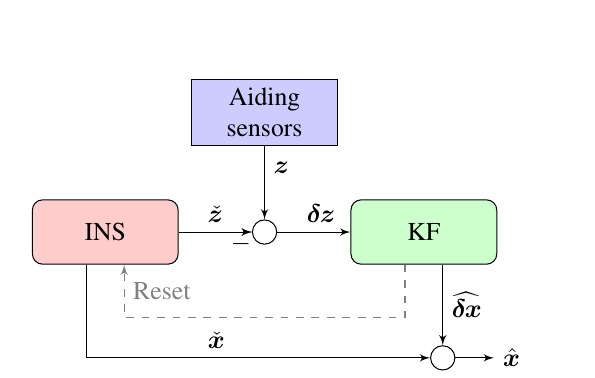
\includegraphics[scale=1.0]{/home/rohan/Documents/thesis_work/model_aided_intertial_nvaigation_system_traditional.png}
\end{figure}

\begin{figure}[hbtp]
\caption{Traditional aided INS}
\centering
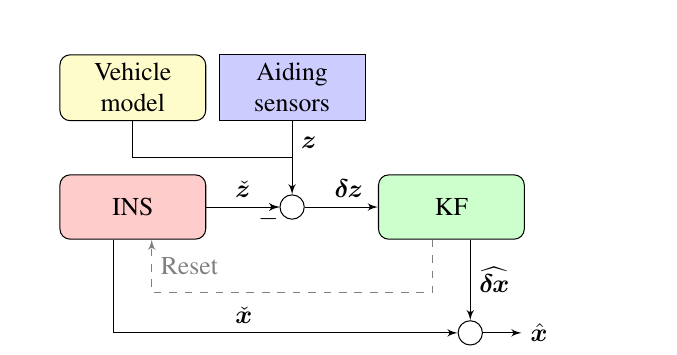
\includegraphics[scale=1.0]{/home/rohan/Documents/thesis_work/model_aided_intertial_nvaigation_system_model.png}
\end{figure}
In the traditional aided INS the readings from gyro and accelerometer measurements from the IMU are integrated over time to give an estimate of velocity,position and orientation. Due to the inherent errors in the gyros and accelerometers there is a drift in  the INS system. There are aiding sensors such as DVL and surface GPS to compensate the drift for the IMU. The reading from the sensors are fused using a Bayes filters to get an enchained estimate of velocity ,position and orientation. 

In the model aided INS the IMU suffers from the same drift but the output from the model is treated analogously to that of an external aiding sensor. In this system the DVL in traditional INS systems are replaced by vehicle model. The output from the model i.e. the velocity estimate is fused with the readings from the INS by a Bayes filter. The integrating of vehicle model with the IMU systems help in systems which lack external velocity measurements. The other implication is in systems where redundancy and integrity is important e.g. during sensor drop outs or sensor failures.

This specific application shows the importance of having a accurate motion model. As stated in earlier chapters the motion model can change due to various factors and would have a direct impact on the navigation systems of underwater vehicles.Wrong estimates from the motion model will not benefit INS systems and overall lead to wrong estimate about the position and orientation of the vehicle. Our algorithm shows on how to learn the motion model on the fly which can lead to better estimate of the velocity and therefore accurate navigation systems.

As you can see in the figure the input to the motion model is a control command and output is the velocity estimate. In HUGIN 4500 they had implemented a static motion model as table look up based on experimental data i.e.
$u_{r}=f(n_{s})$  where $n_{s}$ is the control system set point. The velocity estimate $u_{r}$ is fused with the reading from IMU to get a better estimate of the position of the AUV. As shown before we try to learn the motion model to find the best estimate for the velocity so that it can aid the INS in this particular application. 

\section{Results}
\label{results}
We use a simulation to demonstrate the effectiveness of learning the
motion model. The simulation mainly consists of particle filter SLAM.
We use a motion model described in the above chapters. The sensor
model basically measures the distance from the four static landmarks
defined at the start of the experiment. The experiment runs over 100
time steps and at every 5\textsuperscript{th} time step we change
the parameters of the motion model. As described in the above chapters
the parameters that we intended to learn are $\sigma_{D_{d}}^{2}$,$\sigma_{T_{d}}^{2}$,$\sigma_{D_{1}}^{2},\sigma_{D_{r}}^{2}$,$\sigma_{T_{r}}^{2}$,$\sigma_{D_{1}}^{2}$,$\sigma_{T_{1}}^{2}$.
In the first stage of the experiment at every 5\textsuperscript{th }time step
we change $\sigma_{D_{d}}^{2}$ or $\sigma_{T_{r}}^{2}$in our motion
model. The following table and plots describes the five experiments
that were conducted in the simulation.

\begin{tabular}{|c|c|c|c|c|c|}
\hline 
No. & $\sigma_{D_{d}}$ & $\sigma_{T_{r}}$ & $\sigma_{D_{d}}^{*}$ & $\sigma_{T_{r}}^{*}$ & Sensor Noise\tabularnewline
\hline 
\hline 
1 & 0.05 & 0.05 & 0.2 & 0.05 & 2.0\tabularnewline
\hline 
2 & 0.05 & 0.05 & 0.2 & 0.05 & 5.0\tabularnewline
\hline 
4 & 0.05 & 0.05 & 0.5 & 0.05 & 2.0\tabularnewline
\hline 
5 & 0.05 & 0.05 & 0.5 & 0.05 & 5.0\tabularnewline
\hline 
6 & 0.05 & 0.05 & 0.05 & 0.2 & 5.0\tabularnewline
\hline 
7 & 0.05 & 0.05 & 0.05 & 0.5 & 5.0\tabularnewline
\hline 
\end{tabular}
\\

$\sigma_{D_{d}}$,$\sigma_{T_{r}}$ are the parameters values that
the motion model was initialized. These values are altered in order
to simulate a change in the motion model and they are described by
$\sigma_{D_{d}}^{*}$,$\sigma_{T_{r}}^{*}$. The sensor noise can
be described as the confidence the robot has in its sensor model .
The impact of the noise on the localization error can be seen in the
following plots.	

\begin{figure}
\caption{$\sigma_{D_{d}}$=0.05 $\sigma_{D_{d}}^{*}$ = 0.2 Sensor Noise= 2.0}


\includegraphics[scale=0.25]{\lyxdot \lyxdot /plot_motion_model/100_0\lyxdot 05_0\lyxdot 2_1_2\lyxdot 0_motion_model_1}
\end{figure}


\begin{figure}
\caption{$\sigma_{D_{d}}$=0.05 $\sigma_{D_{d}}^{*}$ = 0.2 Sensor Noise= 5.0}


\includegraphics[scale=0.25]{\lyxdot \lyxdot /plot_motion_model/100_0\lyxdot 05_0\lyxdot 2_1_5\lyxdot 0_motion_model_1}

\end{figure}


Figure 1 and Figure 2 are plots of the localization error with different
sensor noises. We can see in both the cases the learned motion model
performed better than the static motion model. Another important point
is that the average error is less when the sensor noise is 2.0 as
compared to the second case. This can be accounted for the fact that
our localization algorithm is more confident on the sensor model as
compared to the motion model. 

\begin{figure}
\caption{$\sigma_{D_{d}}$=0.05 $\sigma_{D_{d}}^{*}$ = 0.5 Sensor Noise= 2.0}


\includegraphics[scale=0.25]{\lyxdot \lyxdot /plot_motion_model/100_0\lyxdot 05_0\lyxdot 5_1_2\lyxdot 0_motion_model}

\end{figure}


\begin{figure}
\caption{$\sigma_{D_{d}}$=0.05 $\sigma_{D_{d}}^{*}$ = 0.5 Sensor Noise= 5.0}


\includegraphics[scale=0.25]{\lyxdot \lyxdot /plot_motion_model/100_0\lyxdot 05_0\lyxdot 5_1_5\lyxdot 0_motion_model_1}

\end{figure}


As we can see in Figure 3 and Figure 4 at 5\textsuperscript{th} time
step the error shooting up but the learned motion model brings back
the error whereas the static motion model takes time to recover back
depending upon the sensor noise. In both the figures we can see that
the error is pretty static in the learned motion model whereas in
the static motion model there is a lot of fluctulation. 

\begin{figure}
\caption{$\sigma_{T_{r}}$=0.05 $\sigma_{T_{r}}^{*}$ = 0.2 Sensor Noise= 5.0}


\includegraphics[scale=0.75]{\lyxdot \lyxdot /plot_motion_model/100_0\lyxdot 05_0\lyxdot 2_rotation_5\lyxdot 0_motion_model}

\end{figure}


\begin{figure}
\caption{$\sigma_{T_{r}}$=0.05 $\sigma_{T_{r}}^{*}$ = 0.5 Sensor Noise= 5.0}


\includegraphics[scale=0.25]{\lyxdot \lyxdot /plot_motion_model/100_0\lyxdot 05_0\lyxdot 5_rotation_5\lyxdot 0_motion_model}

\end{figure}


Figure 5 and Figure 6 describe the errors when the robot rotational
motion is much more than the translational motion. We can clearly
see that the learned motion model quickly adapts to the changes whereas
the static motion model struggles to get the error down. 

In all the cases it was very clear that we could see the adaptive
motion model performing better than the static. The sensor noise had
its impact on the overall error. Robot calibration is important to
process in mobile robotics. The proposed algorithm is an automated
process which can help us in better navigation of the robots and can
be used for any motion model. 

\chapter{Conclusion}

Did it!

\bibliographystyle{plain}
\bibliography{mendeley.bib}

\end{document}
